

%%%%%%%%%%%%%%%%%%%%%
\section{Perspective et repère SiCP}
%%%%%%%%%%%%%%%%%%%%%
Cette section traite de la définition des coordonnées intervenant dans la projection en perspective de SiCP
\subsection{Schéma}
%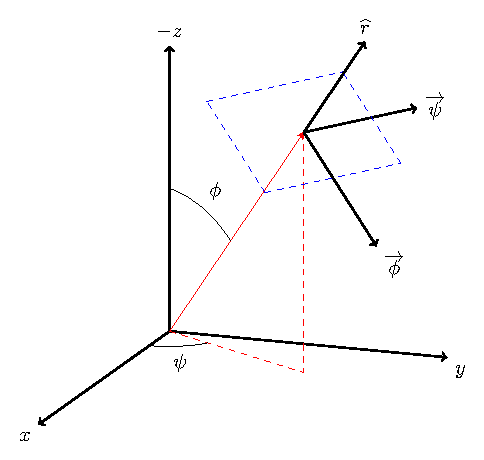
\includepdf{./illustration/repereSiCP.pdf}
\begin{figure}
	\begin{minipage}[c]{.46\linewidth}
	$\overrightarrow{r}  = \text{} .
	\begin{pmatrix}
		\cos \psi . \sin \phi \\
		\sin \psi . \sin \phi \\
		\cos \phi
	\end{pmatrix}$,

	$\overrightarrow{\psi} = \text{largeur} .
	\begin{pmatrix}
		- \sin \psi \\
		\cos \psi \\
		0
	\end{pmatrix}$,

	$\overrightarrow{\phi} = \text{hauteur} .
	\begin{pmatrix}
		- \cos \psi . \cos \phi \\
		- \sin \psi . \cos \phi \\
		\sin \phi
	\end{pmatrix}$.
	\end{minipage} \hfill
	\begin{minipage}[c]{.46\linewidth}
	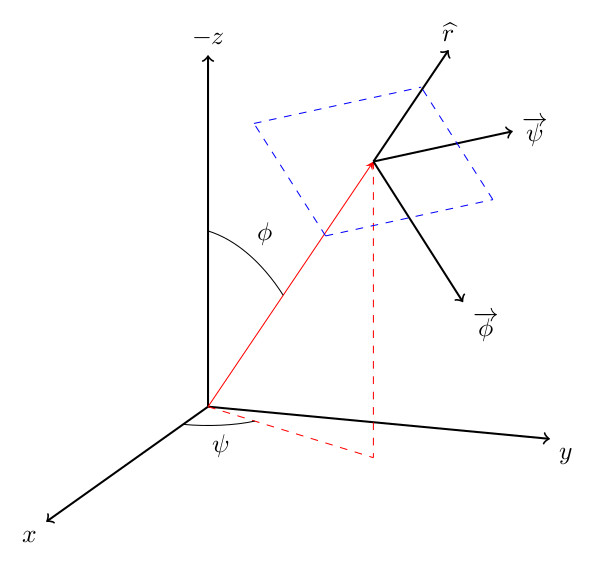
\includegraphics[scale=1]{./illustration/repereSiCP}
	\end{minipage}
\end{figure}
%
%
\begin{center}
 de SiCP
\end{center}


\subsection{Mathématique}
\begin{description}[leftmargin=0.1cm, itemsep=5pt]
\item{\bf System} : $\theta _\text{i}$.
\item{\bf Chaine} : {\bf r}$_\text{i}$.
\item{\bf Support} : {\bf R}$_\text{i}$.
\item{\bf Point de vue} : {\bf M}, {\bf i}$_\text{M}$,
                                   {\bf j}$_\text{M}$,
                                   {\bf k}$_\text{M}$.
\end{description}
\subsection{Classes}
\begin{description}[leftmargin=0.1cm, itemsep=5pt]
\item{\bf System} : nouveau[N].
\item{\bf Chaine} : chaine[N], support[12], largeur, hauteur.
\item{\bf Point de vue} : perspective, distance, psi, phi.
\end{description}
\subsection{Projection}
\begin{description}[leftmargin=0.1cm, itemsep=5pt]
\item{\bf System-Chaine} : r$_\text{i} = 
	\begin{pmatrix}
		\text{largeur} / 2 \text{N} ( \text{i} - \text{N} / 2 ) \\
		\text{hauteur}. \sin \theta _\text{i} \\
		\text{hauteur}. \cos \theta _\text{i}
	\end{pmatrix}$.
\item{\bf Point de vue} : 
	$\overrightarrow{r}  = \text{} .
	\begin{pmatrix}
		\cos \psi . \sin \phi \\
		\sin \psi . \sin \phi \\
		\cos \phi
	\end{pmatrix}$,
	$\overrightarrow{\psi} = \text{largeur} .
	\begin{pmatrix}
		- \sin \psi \\
		\cos \psi \\
		0
	\end{pmatrix}$,
	$\overrightarrow{\phi} = \text{hauteur} .
	\begin{pmatrix}
		- \cos \psi . \cos \phi \\
		- \sin \psi . \cos \phi \\
		\sin \phi
	\end{pmatrix}$.
\item{\bf Chaine-Rendu} : $\text{g}_\text{i} = 
	\begin{pmatrix}
	(\text{\bf r}_\text{i} - \text{\bf M}).{\text{\bf k}}_\text{M} + \text{hauteur} / 2 \\
	(\text{\bf r}_\text{i} - \text{\bf M}).{\text{\bf j}}_\text{M} + \text{largeur} / 2
	\end{pmatrix}$.
\end{description}
%%%%%%%%%%%%%%%%%%%%%%%%%%%%%%%%%%%%%%%%%%%%%%%%%%%%%%%%%%%%%%%%%%%%%%%%%%%%%%%%%%%%%
